\documentclass{ximera}

%\usepackage{todonotes}

\newcommand{\todo}{}

\usepackage{tkz-euclide}
\tikzset{>=stealth} %% cool arrow head
\tikzset{shorten <>/.style={ shorten >=#1, shorten <=#1 } } %% allows shorter vectors

\usepackage{tkz-tab}  %% sign charts
\usetikzlibrary{decorations.pathreplacing} 

\usetikzlibrary{backgrounds} %% for boxes around graphs
\usetikzlibrary{shapes,positioning}  %% Clouds and stars
\usetikzlibrary{matrix} %% for matrix
\usepgfplotslibrary{polar} %% for polar plots
\usetkzobj{all}
\usepackage[makeroom]{cancel} %% for strike outs
%\usepackage{mathtools} %% for pretty underbrace % Breaks Ximera
\usepackage{multicol}

\usepackage{polynom}



\usepackage[many]{tcolorbox}  %% for titled boxes
\newtcolorbox{xbox}[1]{%
    tikznode boxed title,
    enhanced,
    arc=0mm,
    interior style={white},
    attach boxed title to top center= {yshift=-\tcboxedtitleheight/2},
    fonttitle=\bfseries,
    colbacktitle=white,coltitle=black,
    boxed title style={size=normal,colframe=white,boxrule=0pt},
    title={#1}}


\usepackage{array}
\setlength{\extrarowheight}{+.1cm}   
\newdimen\digitwidth
\settowidth\digitwidth{9}
\def\divrule#1#2{
\noalign{\moveright#1\digitwidth
\vbox{\hrule width#2\digitwidth}}}





\newcommand{\RR}{\mathbb R}
\newcommand{\R}{\mathbb R}
\newcommand{\N}{\mathbb N}
\newcommand{\Z}{\mathbb Z}

%\renewcommand{\d}{\,d\!}
\renewcommand{\d}{\mathop{}\!d}
\newcommand{\dd}[2][]{\frac{\d #1}{\d #2}}
\newcommand{\pp}[2][]{\frac{\partial #1}{\partial #2}}
\renewcommand{\l}{\ell}
\newcommand{\ddx}{\frac{d}{\d x}}
\newcommand{\ddt}{\frac{d}{\d t}}

\newcommand{\zeroOverZero}{\ensuremath{\boldsymbol{\tfrac{0}{0}}}}
\newcommand{\inftyOverInfty}{\ensuremath{\boldsymbol{\tfrac{\infty}{\infty}}}}
\newcommand{\zeroOverInfty}{\ensuremath{\boldsymbol{\tfrac{0}{\infty}}}}
\newcommand{\zeroTimesInfty}{\ensuremath{\small\boldsymbol{0\cdot \infty}}}
\newcommand{\inftyMinusInfty}{\ensuremath{\small\boldsymbol{\infty - \infty}}}
\newcommand{\oneToInfty}{\ensuremath{\boldsymbol{1^\infty}}}
\newcommand{\zeroToZero}{\ensuremath{\boldsymbol{0^0}}}
\newcommand{\inftyToZero}{\ensuremath{\boldsymbol{\infty^0}}}



\newcommand{\numOverZero}{\ensuremath{\boldsymbol{\tfrac{\#}{0}}}}
\newcommand{\dfn}{\textbf}
%\newcommand{\unit}{\,\mathrm}
\newcommand{\unit}{\mathop{}\!\mathrm}
\newcommand{\eval}[1]{\bigg[ #1 \bigg]}
\newcommand{\seq}[1]{\left( #1 \right)}
\renewcommand{\epsilon}{\varepsilon}
\renewcommand{\iff}{\Leftrightarrow}

\DeclareMathOperator{\arccot}{arccot}
\DeclareMathOperator{\arcsec}{arcsec}
\DeclareMathOperator{\arccsc}{arccsc}
\DeclareMathOperator{\si}{Si}
\DeclareMathOperator{\proj}{proj}
\DeclareMathOperator{\scal}{scal}


\newcommand{\tightoverset}[2]{% for arrow vec
  \mathop{#2}\limits^{\vbox to -.5ex{\kern-0.75ex\hbox{$#1$}\vss}}}
\newcommand{\arrowvec}[1]{\tightoverset{\scriptstyle\rightharpoonup}{#1}}
\renewcommand{\vec}{\mathbf}
\newcommand{\veci}{\vec{i}}
\newcommand{\vecj}{\vec{j}}
\newcommand{\veck}{\vec{k}}
\newcommand{\vecl}{\boldsymbol{\l}}

\newcommand{\dotp}{\bullet}
\newcommand{\cross}{\boldsymbol\times}
\newcommand{\grad}{\boldsymbol\nabla}
\newcommand{\divergence}{\grad\dotp}
\newcommand{\curl}{\grad\cross}
%\DeclareMathOperator{\divergence}{divergence}
%\DeclareMathOperator{\curl}[1]{\grad\cross #1}


\colorlet{textColor}{black} 
\colorlet{background}{white}
\colorlet{penColor}{blue!50!black} % Color of a curve in a plot
\colorlet{penColor2}{red!50!black}% Color of a curve in a plot
\colorlet{penColor3}{red!50!blue} % Color of a curve in a plot
\colorlet{penColor4}{green!50!black} % Color of a curve in a plot
\colorlet{penColor5}{orange!80!black} % Color of a curve in a plot
\colorlet{fill1}{penColor!20} % Color of fill in a plot
\colorlet{fill2}{penColor2!20} % Color of fill in a plot
\colorlet{fillp}{fill1} % Color of positive area
\colorlet{filln}{penColor2!20} % Color of negative area
\colorlet{fill3}{penColor3!20} % Fill
\colorlet{fill4}{penColor4!20} % Fill
\colorlet{fill5}{penColor5!20} % Fill
\colorlet{gridColor}{gray!50} % Color of grid in a plot

\newcommand{\surfaceColor}{violet}
\newcommand{\surfaceColorTwo}{redyellow}
\newcommand{\sliceColor}{greenyellow}




\pgfmathdeclarefunction{gauss}{2}{% gives gaussian
  \pgfmathparse{1/(#2*sqrt(2*pi))*exp(-((x-#1)^2)/(2*#2^2))}%
}


%%%%%%%%%%%%%
%% Vectors
%%%%%%%%%%%%%

%% Simple horiz vectors
\renewcommand{\vector}[1]{\left\langle #1\right\rangle}


%% %% Complex Horiz Vectors with angle brackets
%% \makeatletter
%% \renewcommand{\vector}[2][ , ]{\left\langle%
%%   \def\nextitem{\def\nextitem{#1}}%
%%   \@for \el:=#2\do{\nextitem\el}\right\rangle%
%% }
%% \makeatother

%% %% Vertical Vectors
%% \def\vector#1{\begin{bmatrix}\vecListA#1,,\end{bmatrix}}
%% \def\vecListA#1,{\if,#1,\else #1\cr \expandafter \vecListA \fi}

%%%%%%%%%%%%%
%% End of vectors
%%%%%%%%%%%%%

%\newcommand{\fullwidth}{}
%\newcommand{\normalwidth}{}



%% makes a snazzy t-chart for evaluating functions
%\newenvironment{tchart}{\rowcolors{2}{}{background!90!textColor}\array}{\endarray}

%%This is to help with formatting on future title pages.
\newenvironment{sectionOutcomes}{}{} 



%% Flowchart stuff
%\tikzstyle{startstop} = [rectangle, rounded corners, minimum width=3cm, minimum height=1cm,text centered, draw=black]
%\tikzstyle{question} = [rectangle, minimum width=3cm, minimum height=1cm, text centered, draw=black]
%\tikzstyle{decision} = [trapezium, trapezium left angle=70, trapezium right angle=110, minimum width=3cm, minimum height=1cm, text centered, draw=black]
%\tikzstyle{question} = [rectangle, rounded corners, minimum width=3cm, minimum height=1cm,text centered, draw=black]
%\tikzstyle{process} = [rectangle, minimum width=3cm, minimum height=1cm, text centered, draw=black]
%\tikzstyle{decision} = [trapezium, trapezium left angle=70, trapezium right angle=110, minimum width=3cm, minimum height=1cm, text centered, draw=black]


\outcome{Use limits to find the slope of the tangent line at a point.}
\outcome{Understand the definition of the derivative at a point.}
\outcome{Compute the derivative of a function at a point.}
\outcome{Write the equation of the tangent line to a graph at a given point.}
\outcome{Recognize and distinguish between secant and tangent lines.}

\author{Nela Lakos \and Kyle Parsons}

\begin{document}
\begin{exercise}

The graph of the function $f(x) = \frac{10}{x+2}$ is given below.

\begin{image}
  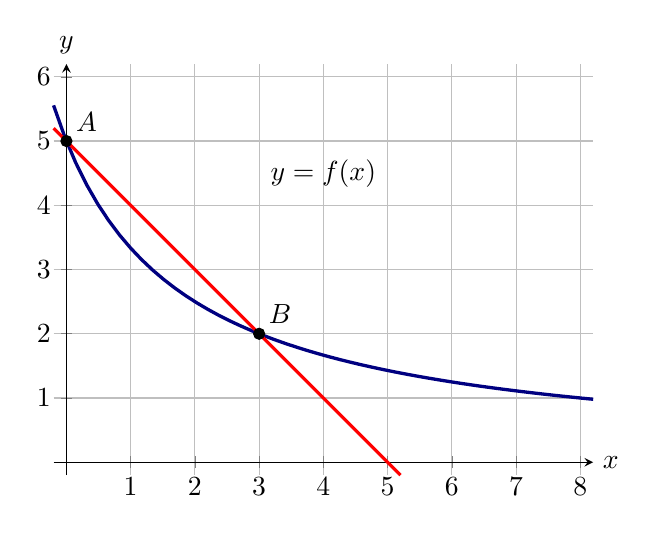
\begin{tikzpicture}
    \begin{axis}[
        xmin=-0.2,xmax=8.2,ymin=-0.2,ymax=6.2,
        clip=false,
        unit vector ratio*=1 1 1,
        axis lines=center,
        grid = major,
        ytick={0,1,...,6},
    xtick={0,1,...,8},
        xlabel=$x$, ylabel=$y$,
        every axis y label/.style={at=(current axis.above origin),anchor=south},
        every axis x label/.style={at=(current axis.right of origin),anchor=west},
      ]
		\addplot[very thick,penColor,domain=-0.2:8.2,samples=50] plot{10/(x+2)};
		
		\addplot[only marks,mark=*] coordinates{(0,5) (3,2)};
		\node at (axis cs:0,5) [above right] {$A$};
		\node at (axis cs:3,2) [above right] {$B$};
		
		\addplot[very thick,red,domain=-0.2:5.2] plot{5-x};
		
		\node at (axis cs:4,4.5) {$y=f(x)$};

      \end{axis}`
  \end{tikzpicture}
\end{image}

Let $A$ and $B$ be two points on the graph of $f$ as depicted above.
\[
A  = \left(0,\answer{5}\right) \quad B = \left(3,\answer{2}\right)
\]

\begin{exercise}

The slope, $m_{\text{sec}}$, of the secant line through the points $A$ and $B$ is
\[
m_{\text{sec}} = \answer{-1}.
\]

\begin{exercise}

The figure below depicts the tangent line to the curve $y=f(x)$ at the point B.

\begin{image}
  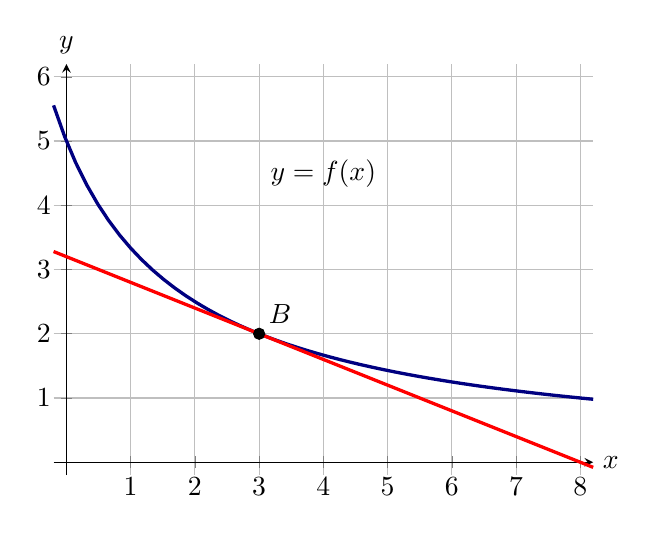
\begin{tikzpicture}
    \begin{axis}[
        xmin=-0.2,xmax=8.2,ymin=-0.2,ymax=6.2,
        clip=false,
        unit vector ratio*=1 1 1,
        axis lines=center,
        grid = major,
        ytick={0,1,...,6},
    xtick={0,1,...,8},
        xlabel=$x$, ylabel=$y$,
        every axis y label/.style={at=(current axis.above origin),anchor=south},
        every axis x label/.style={at=(current axis.right of origin),anchor=west},
      ]
		\addplot[very thick,penColor,domain=-0.2:8.2,samples=50] plot{10/(x+2)};
		
		\addplot[only marks,mark=*] coordinates{(3,2)};
		\node at (axis cs:3,2) [above right] {$B$};
		
		\addplot[very thick,red,domain=-0.2:8.2] plot{-2/5*(x-3)+2};
		
		\node at (axis cs:4,4.5) {$y=f(x)$};

      \end{axis}`
  \end{tikzpicture}
\end{image}

The slope of the tangent line to the curve $y=f(x)$ at the point $(a,f(a))$ is given by
\[
m_{\text{tan}} = \lim_{x\to a}\frac{f(x)-f(a)}{x-a},
\]
provided the limit exists.

Using the definition above, the slope of the tangent line to $y=f(x)$ at the point $B$ is
\[
m_{\text{tan}} = \answer{\frac{-2}{5}}.
\]

\begin{exercise}

The equation of the tangent line to $y=f(x)$ at the point $B$ is
\[
y=\answer{-\frac{2}{5}(x-3)+2}.
\]

\end{exercise}
\end{exercise}
\end{exercise}
\end{exercise}
\end{document}